\problemname{Tabs and spaces}

\begin{wrapfigure}{r}{0.4\textwidth}
    \centering
    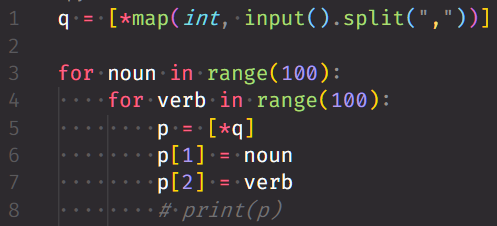
\includegraphics[width=0.4\textwidth]{code}
\end{wrapfigure}

\noindent
Picture this. Your favourite code repository hosting site is hosting a conference at
Chalmers. And you've gone to it. They've talked about a bunch of fun stuff like
merge conflicts, accidentally discarding your changes and someone force-pushing
their commit over yours so that all your work just goes to waste. They also
brought up the importance of efficient text compression. Something about how if
everyone indented their code with tabs instead of spaces, they would save a
colossal amount of space.  But at that point you weren't really concentrating,
since you knew there was going to be free lunch and you were starving.

After you get home, you check your own code. You realise, it's all indented
with spaces! And every single space takes up a whole byte. \textit{A whole
byte!} Disgusted by this pointless waste of storage space, you convert all of
your files to use tabs for indentation. But then you start to think. What
if\ldots tabs weren't specifically four spaces wide? What if you could save even
more space if tabs were some other width? You immediately get to work solving
this problem.

\section*{Input}

The input begins with one number $F$, the amount of files in your project. Then
follow $F$ files. Each file begins with a number $L$, the lines in your
program. Each following ``line'' is represented by a number $N$, the amount of
spaces used to indent that line. Your project can have up to $10$ files, each
with up to $20$ lines. Oh, and your project is written in Python, so the line length
can be up to $80$ of which $79$ characters can be spaces. (You're a PEP abiding code
golfer.)

\section*{Output}

Print two numbers, one on each line. First the width of your custom tab symbol
in spaces, then the total amount of space saved in bytes.

\section*{Things to note}

Your code still has to look the same after you've substituted some of the spaces
with tabs. If you find two or more tab sizes that save the same amount of space,
pick the smaller one. Tabs also have to be at least one space wide.
